% ORF Prediction
%
% An example of ORF prediction, using Artemis.
% This is a long subsection, so we break it up further with subsections 
% and subsubsections

\subsection{ORF Prediction}
\subsubsection{Introduction}
\begin{frame}
  \frametitle{ORF Prediction}
  \begin{itemize}
    \item Open Reading Frame = sequence between successive stop codons
    \item A very naive method - unsupervised \textit{de novo} prediction
    \item Sufficiently long ORFs are genes (or exons)
    \item Many tools:
    \begin{itemize}
      \item Artemis
      \item EMBOSS \texttt{getorf}
      \item hundreds of ``in-house'' scripts$\ldots$
    \end{itemize}
  \end{itemize}
\end{frame}

\subsubsection{Generate Initial Candidate Set}
\begin{frame}
  \frametitle{Mark ORFs in Artemis}    
  \begin{center}
    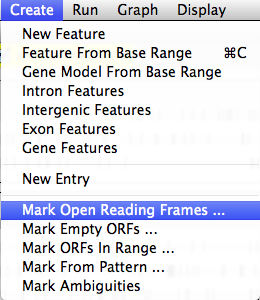
\includegraphics[width=0.4\textwidth]{images/artemis_orf0}     
  \end{center}
\end{frame}

\begin{frame}
  \frametitle{Select Minimum Reading Frame Size}
  Biological insight required: what size should the smallest ORF be?
  \begin{center}
    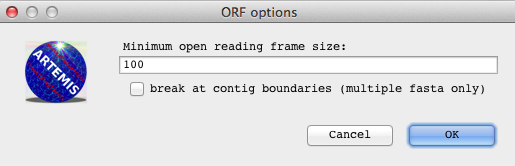
\includegraphics[width=0.9\textwidth]{images/artemis_orf1}     
  \end{center}
\end{frame}

\begin{frame}
  \frametitle{Forward ID}    
  \begin{center}
    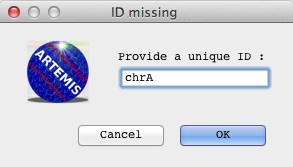
\includegraphics[width=0.9\textwidth]{images/artemis_orf2}     
  \end{center}
\end{frame}

\begin{frame}
  \frametitle{Reverse ID}    
  \begin{center}
    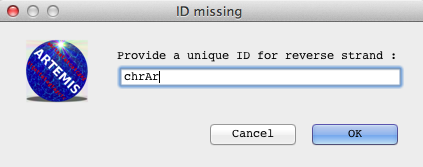
\includegraphics[width=0.9\textwidth]{images/artemis_orf3}     
  \end{center}
\end{frame}

\begin{frame}
  \frametitle{First Candidate Set} 
  Is this good enough?
  \begin{center}
    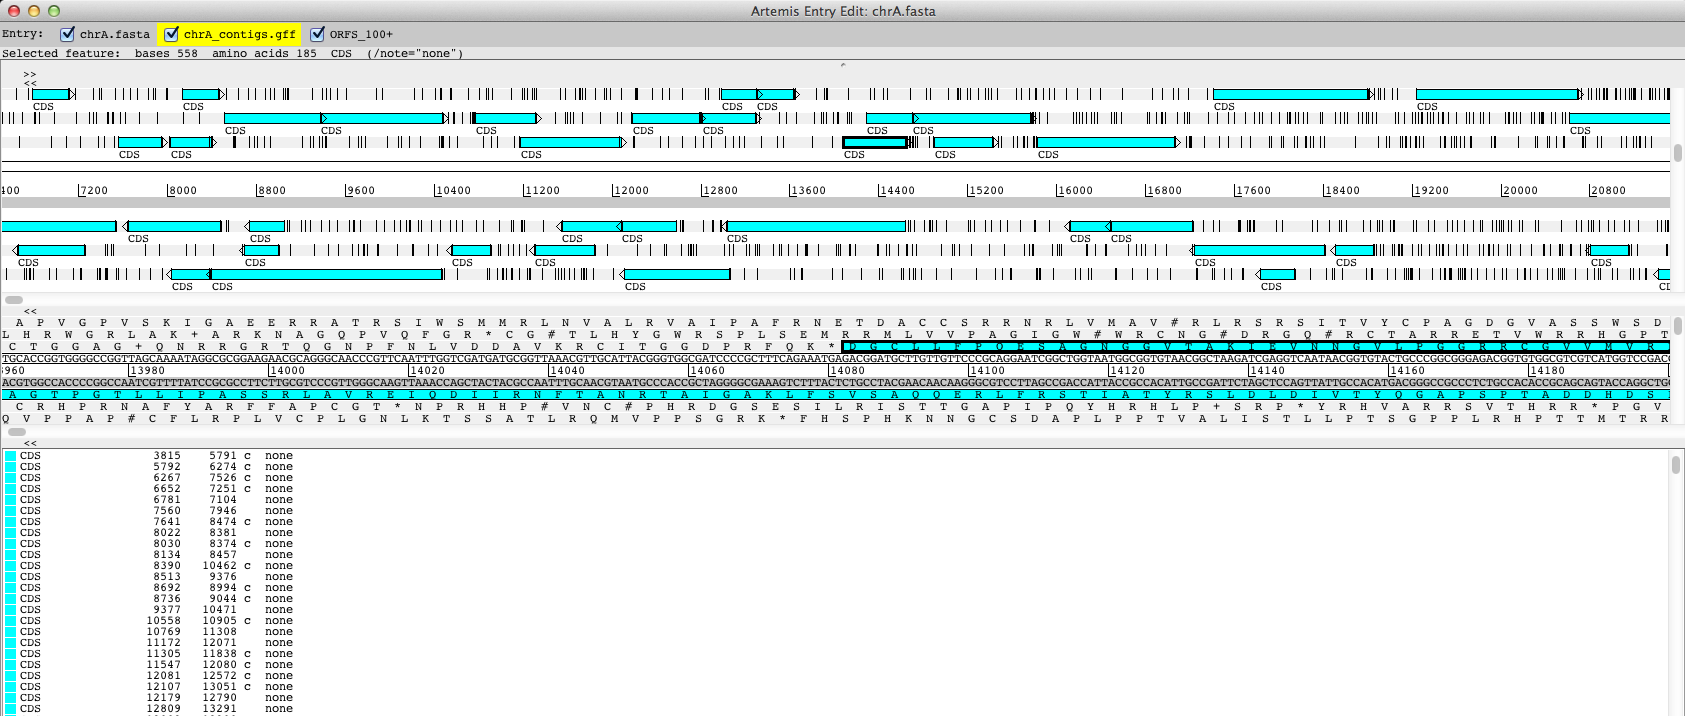
\includegraphics[width=0.9\textwidth]{images/artemis_orf4}     
  \end{center}
\end{frame}

\subsection{Trim First Prediction Set}
\begin{frame}
  \frametitle{View Predicted Sequence}    
  \begin{center}
    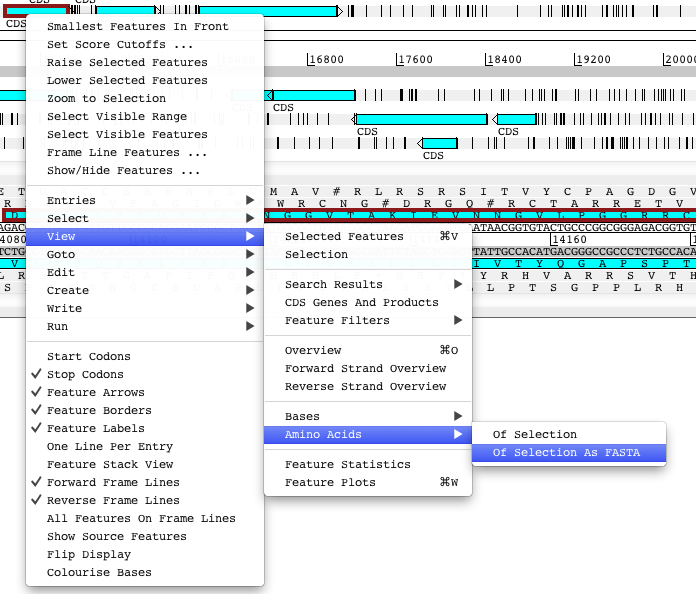
\includegraphics[width=0.7\textwidth]{images/artemis_orf5}     
  \end{center}
\end{frame}

\begin{frame}
  \frametitle{ORF $\neq$ CDS}
  Biological insight: CDS start with start codon.
  \begin{center}
    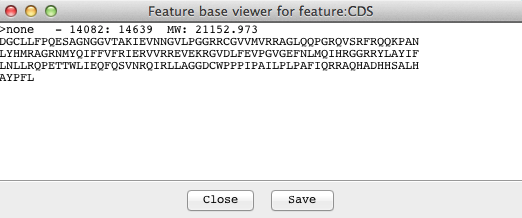
\includegraphics[width=0.9\textwidth]{images/artemis_orf6}     
  \end{center}
\end{frame}

\begin{frame}
  \frametitle{Select All Predictions}    
  \begin{center}
    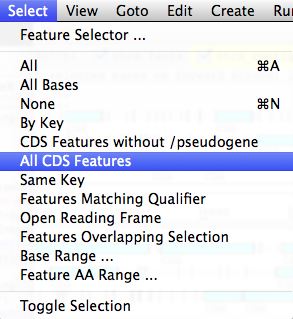
\includegraphics[width=0.5\textwidth]{images/artemis_orf7}     
  \end{center}
\end{frame}

\begin{frame}
  \frametitle{Trim to First Met}    
  \begin{center}
    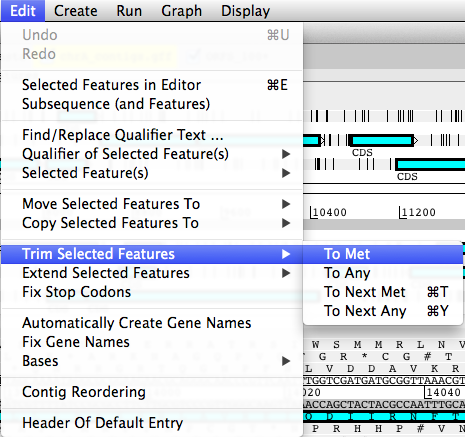
\includegraphics[width=0.6\textwidth]{images/artemis_orf8}     
  \end{center}
\end{frame}

\begin{frame}
  \frametitle{Failures}
  What does this mean, in terms of biology?
  \begin{center}
    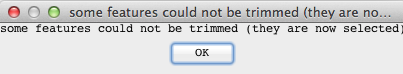
\includegraphics[width=0.9\textwidth]{images/artemis_orf9}     
  \end{center}
\end{frame}

\begin{frame}
  \frametitle{Delete Failures}    
  \begin{center}
    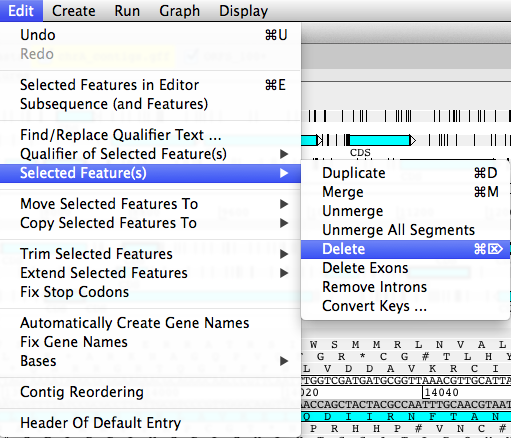
\includegraphics[width=0.6\textwidth]{images/artemis_orf10}     
  \end{center}
\end{frame}

\subsection{Assess Second Prediction Set}
\begin{frame}
  \frametitle{Assess Performance} 
  5410 ORFs with no start codon - how good is ORF detection at finding CDS?
  \begin{center}
    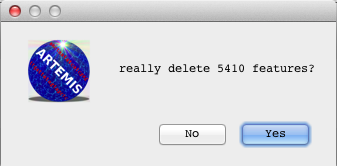
\includegraphics[width=0.9\textwidth]{images/artemis_orf11}     
  \end{center}
\end{frame}

\begin{frame}
  \frametitle{Name Predicted CDS}
  Where do gene names come from?
  \begin{center}
    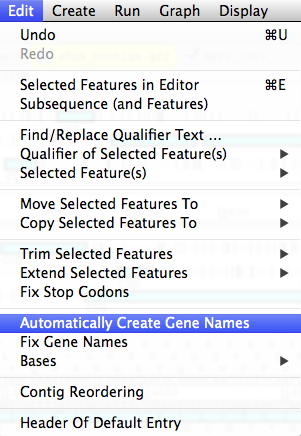
\includegraphics[width=0.3\textwidth]{images/artemis_orf12}     
  \end{center}
\end{frame}

\begin{frame}
  \frametitle{Select Prefix}    
  \begin{center}
    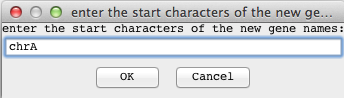
\includegraphics[width=0.9\textwidth]{images/artemis_orf13}     
  \end{center}
\end{frame}

\begin{frame}
  \frametitle{Second Candidate Set}   
  Is this good enough? 
  \begin{center}
    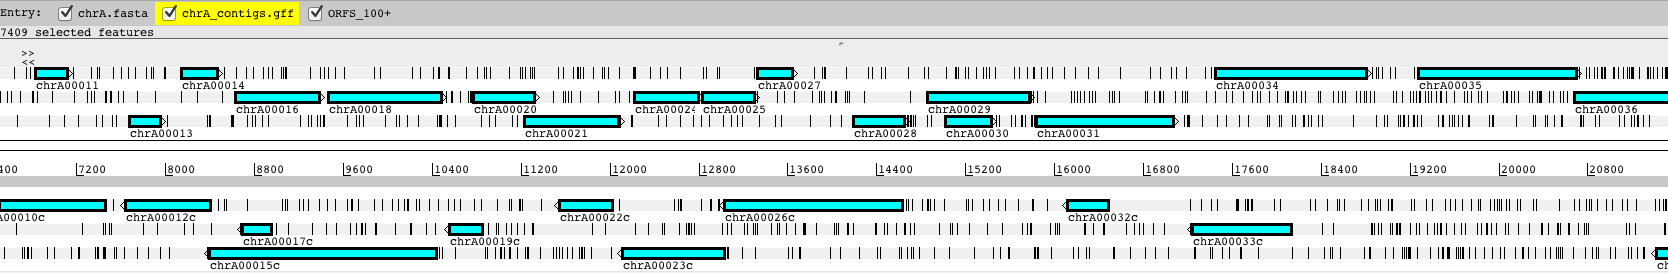
\includegraphics[width=0.9\textwidth]{images/artemis_orf14}     
  \end{center}
  Biological insight: do we expect CDS to overlap like this?
\end{frame}

\subsection{Conclusion}
\begin{frame}
  \frametitle{Lessons learned}   
  \begin{itemize}
    \item ORF finding is very simple, but still requires biological insight and parameter choices
    \item It's not a very precise way to identify genes or CDS (especially in eukaryotes)
    \item Even in prokaryotes, we only get a candidate set of CDS (many spurious) requiring manual refinement
  \end{itemize}
\end{frame}
